
\documentclass[10pt,conference, twocolumn]{IEEEtran}
\hyphenation{op-tical net-works semi-conduc-tor}

\usepackage[utf8]{inputenc}
\usepackage{listings}
\usepackage{color}
\usepackage{kpfonts,dsfont}
\usepackage{graphicx}
\usepackage{float}
\usepackage{algorithm}
\usepackage[noend]{algpseudocode}
\usepackage{amsmath, amsthm, amssymb, amsfonts}
\usepackage{datetime}
\usepackage{listings}
\usepackage{color}
\definecolor{codegreen}{rgb}{0,0.6,0}
\definecolor{codegray}{rgb}{0.5,0.5,0.5}
\definecolor{codepurple}{rgb}{0.58,0,0.82}
\definecolor{backcolour}{rgb}{0.95,0.95,0.92}
\lstdefinestyle{mystyle}{
    backgroundcolor=\color{backcolour},
    commentstyle=\color{codegreen},
    keywordstyle=\color{magenta},
    numberstyle=\tiny\color{codegray},
    stringstyle=\color{codepurple},
    basicstyle=\footnotesize,
    breakatwhitespace=false,
    breaklines=true,
    captionpos=b,
    keepspaces=true,
    numbers=left,
    numbersep=5pt,
    showspaces=false,
    showstringspaces=false,
    showtabs=false,
    tabsize=2
}
\lstset{style=mystyle}


\begin{document}
\title{Langui: Vector Drawing for Scientific Writing}
\author{Jipeng~Wu}
\markboth{CATEGORY, \currenttime, \today}%
{Shell \MakeLowercase{\textit{et al.}}: Using IEEEtran.cls Template!}
\maketitle

\section{Introduction}
\subsection{Purpose of the Final Report}
This report describes (1) how to go through the Langui deliverable, (2) why Langui matters in real world scenario, and therefore is an enterprise computing application rather than a mathematics or algorithm implementation, (3) the architecture of Langui, (4) some design decisions, algorithms and implementation details, (5) usability evaluation and findings on how to improve. 

\subsection{Diagramming Conventions}
Usually it's pretty flexible and thus not worth mentioning. But in this document, all geometric diagrams must be generated by Langui, which makes this report itself a real world application of Langui.

\subsection{Reading Suggestions}
This final deliverable includes (1) the Langui source code, (2) a final report, (3) a user manual, (4) some experiment data, (5) and a presentation elaborating implementation details and algorithms.

You can just go through this report to have a general understanding of Langui project. 

If you are particularly interested in underlying algorithms and what design trade-offs I made, please read the Langui_Implementation_Decisions.pptx slides.

If you are particularly interested in how data that characterizes user input looks like, please refer to the Experiment_Data.xlsx tables. 

If you are interested in implementation, technical details, trivial stuffs like how to customize a html5 canvas, please read the source code. Although it is ninety-five percent a JS project, Langui is actually organized in a readable way. As is shown in Fig.1, it is modularized. The mouse-event framework is implemented in ui.js. The global object Langui and configurations are defined in global.js. The implementation of Langui algorithms are grouped in the core folder. The user-interface related utilities are grouped in the util folder. 

\begin{figure}[H]
\caption{lines and curves}
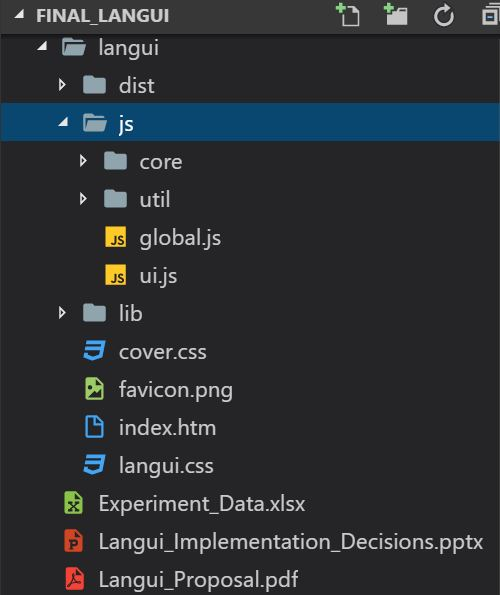
\includegraphics[width=8cm]{w1.JPG}
\end{figure}



\section{Requirement Engineering}

\subsection{Motivation}
Illustrations in research papers can be classified into 2 categories: data-based charts and concept-based illustrations. We don't usually worry about the first one since data-based charts can be generated automatically. The second one howerver could be painful. Those illustrations may not look like existing graphs or figures that diagramming tools already predefined. They usually try to use basic shapes and lines to convey the concept of a novel model. Existing tools like visio, Lucidcharts, metapost, LaTeXDraw or python support such creation.

But sometimes men are too lazy to drag components or write python/R/TikZ/metapost code.

I want to simply draw what it is in my mind and the software should understand my sketches, tidy up everything and produce some beautiful illustrations.

\begin{figure}[H]
\caption{lines and curves}
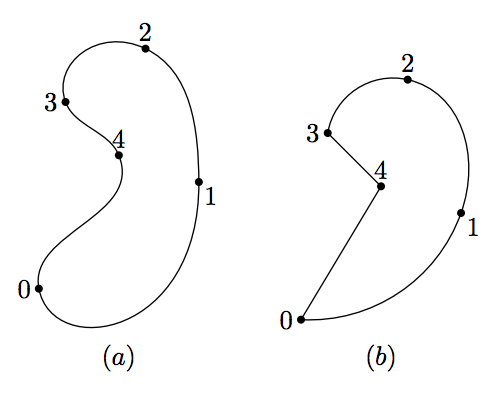
\includegraphics[width=8cm]{1.png}
\end{figure}

\begin{figure}[H]
\caption{arrows and texts}
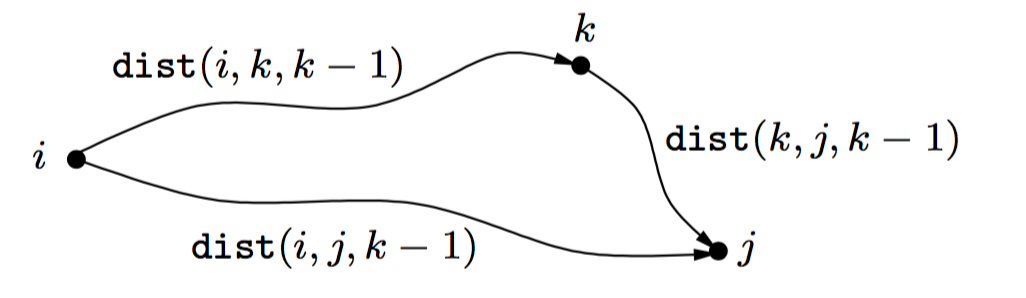
\includegraphics[width=8cm]{2.png}
\end{figure}

\begin{figure}[H]
\caption{basic shapes}
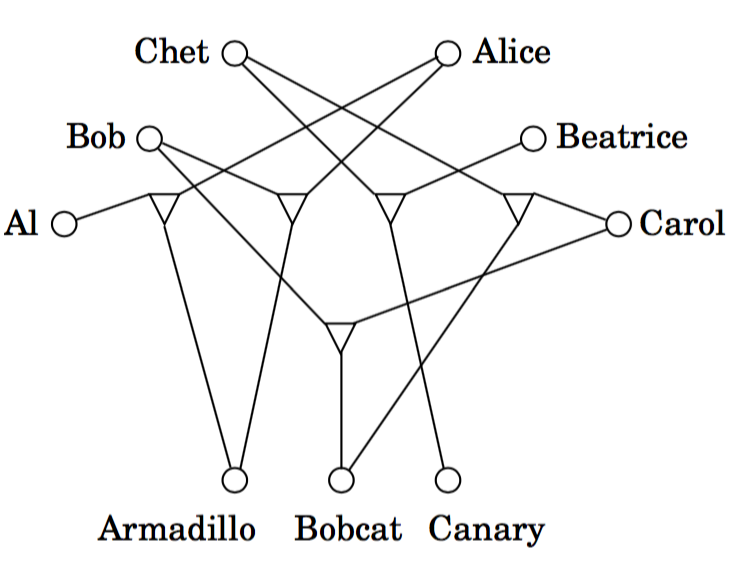
\includegraphics[width=8cm]{3.png}
\end{figure}

\begin{figure}[H]
\caption{overlapping shapes}
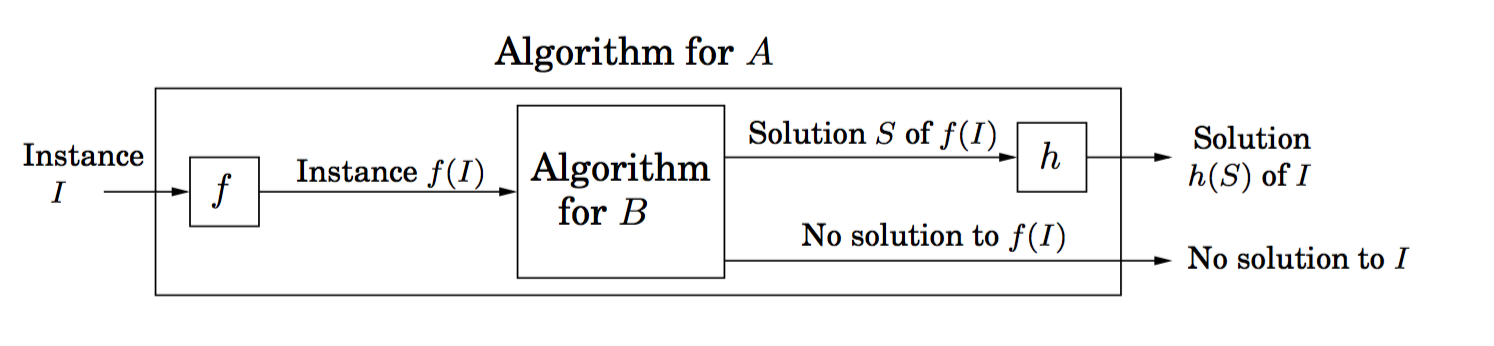
\includegraphics[width=8cm]{4.png}
\end{figure}
\subsection{High level Objectives}

More specifically, it should outperform visio, Lucidchart or code-based tools in efficiency and satisfaction. In terms of completeness and effectiveness, I would not expect full coverage of all features and functions that diagramming tools generally have. However, the Langui program should at least be able to produce the following illustrations: "lines and curves", "arrows and texts", "basic shapes", "overlapping shapes".



\subsection{Goal decomposition and Requirement Elicitation}

A decomposed goal is to develop a tool that understands users' handdrawing and produce illustrations for scientific writing.


\section{Related work}
Existing digramming tools like visio, Lucidcharts provide a wide range of predefined components. Users select an item and then drag it to some place. When they finish drawing one item, the following item is usually different. So they have to search and click another item. This process is very tiring and especially frustrating when you forget to change the selected item.

Selecting and dragging mode will be a submode in Langui. I think it is still necessary to support this mode. So users are allowed to tweak their layouts after drawing the sketches.

I always want to find a tool that tidy things up and magically makes it look professsional. I haven't found anything like that. But I do find similar ideas exploited in gesture understanding and Chinese stroke input method.


\section{Proposed work}

\subsection{Architecture}
\begin{figure}[H]
\caption{Architecture}
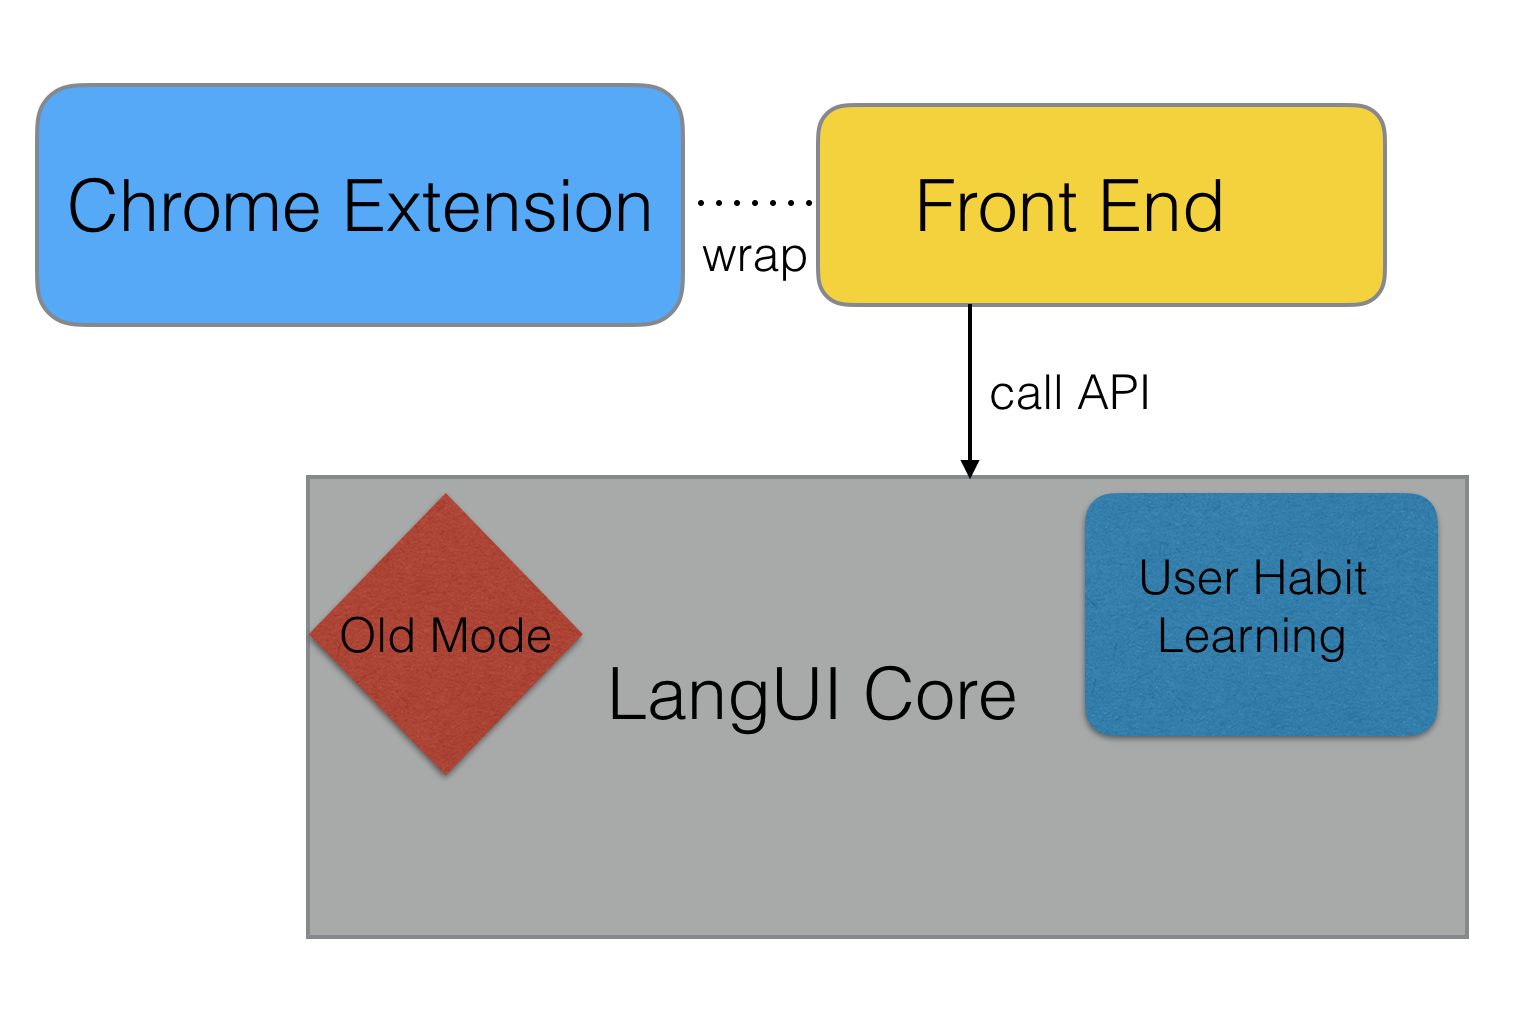
\includegraphics[width=8cm]{5.png}
\end{figure}

Langui is composed of 3 parts: a Google Chrome extension wrapper, a html5 front end and Langui core.

When you write some reports or paper, you are probably using a keyboard and a mouse. So I wouldn't consider tablets even though they are better devices for hand drawing. To make this tool more available,  cross-platform and lightweight, I decide to wrap it as Google Chrome Extension. The front end could be most likely written in html5. But it could change during implementation phase.

The Langui core should provide the following features:

\begin{enumerate}
  \item Understanding users' strokes: Since users draws in Langui's front-end, the speed and direction of strokes can be tracked. Langui can analyze these features to guess the users' intension. For example, I would prefer to draw a "C" or "6" very quickly to embody the concept of "circle", Langui should differentiate these strokes from a slow and smooth "C"/"6"-like curve.
  \item Tidying up the sketches to make them look like computer generated illustrations: Langui should automatically generate smooth curves and straight lines. Automatic aligning is an optional feature.
  \item Old mode: It is the selecting and dragging mode. It is optional, but I do want to finish it as it could be a crucial supplement for the proposed workflow.
  \item Supervised learning: The Langui learning submodule should track and learn users' preference on how to draw certain elements. The data coud be stored on a server and linked to their social media account. But I think simply using cookie is also acceptable in this scenario.  This feature is optional. If I don't have enough time, the default setting would be my personal preference.
\end{enumerate}


\subsection{Algorithms}




\section{Evaluation and Future work}
\subsection{Usablity Analysis}


\subsection{Where I need to Rework or Improve}
It's really hard to beat state-of-the-art diagramming tools in usability. To achieve this goal, I have to make sure Langui's understanding of users' intension is extremely accurate. Any misunderstanding would probably ruin user experience. Therefore the major challenge is how to optimize the stroke understanding module.

\subsection{Critical Future Features}






\section{Bibliography}

\begin{thebibliography}{1}

\bibitem{cmpsim}
 S.W.Draper, \emph{Practical Methods for Measuring Human-Computer Interaction}, Nov 2002. Link: http://www.psy.gla.ac.uk/~steve/resources/uipm.pdf.

\bibitem{mp}
John D. Hobby, \emph{Metapost: A User's Mannual}, May 21, 2014. Link: https://www.tug.org/docs/metapost/mpman.pdf.

\bibitem{ut}
T. Morales de Luna, \emph{Useful Vector Graphic Tools for LATEX Users}, in The PracTEX Journal, 2010, No. 1. Link: https://tug.org/pracjourn/2010-1/morales/morales.pdf.

\end{thebibliography}

\end{document}
